\section{Neural Networks}

Neural networks are a powerful class of models inspired by the human brain, capable of learning complex patterns from data. This section covers their structure, training methods, and advanced applications.

\subsection{Feed-Forward Neural Networks}

Feed-forward neural networks are the foundation of deep learning, consisting of layers of interconnected neurons that process information in one direction.

\mult{2}

\begin{definition}{Neural Network}\\
A neural network is a computational model inspired by the human brain. The basic building block is the neuron, which computes a weighted sum of its inputs, adds a bias term, and applies an activation function:
\[a = \zeta(w^T x + b)\]
where:
\begin{itemize}
    \item $a$ is the neuron's output (activation)
    \item $x$ is the input vector
    \item $w$ is the weight vector
    \item $b$ is the bias
    \item $\zeta$ is the activation function
\end{itemize}
\end{definition}

\begin{definition}{Neuron}\\
    A Neuron applies an activation function to the weighted sum of its inputs\\
    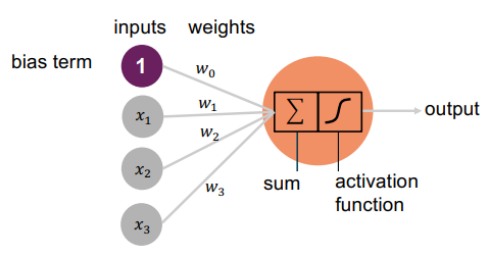
\includegraphics[width=\linewidth]{neuron.png}
\end{definition}

\multend

\begin{definition}{Feed-forward Neural Network}
Feed-forward neural networks consist of neurons organized in layers:
\begin{itemize}
    \item Input layer: Passes input features to the network
    \item Hidden layers: Process information through weighted connections
    \item Output layer: Produces the final prediction
\end{itemize}
Information flows in one direction, from input to output, with no cycles/loops.

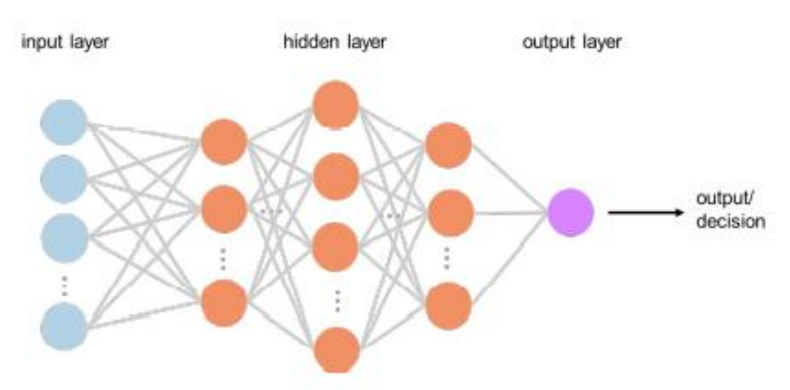
\includegraphics[width=0.6\linewidth]{feed_forward_nn.png}
\end{definition}

\begin{definition}{Softmax Regression}
Softmax regression generalizes logistic regression to multi-class classification:
\begin{itemize}
    \item For each class, it computes a separate linear combination of the inputs
    \item It applies the softmax function to get probabilities for each class: $softmax(z)_k = \frac{\exp(z_k)}{\sum_{i=1}^{K} \exp(z_i)}$
    \item The predicted class is the one with the highest probability
\end{itemize}
\end{definition}

\begin{definition}{Activation Functions}
Common activation functions include:
\begin{itemize}
    \item Sigmoid: $\zeta(z) = \frac{1}{1 + e^{-z}}$, outputs in range (0,1)
    \item Tanh: $\zeta(z) = \frac{e^z - e^{-z}}{e^z + e^{-z}}$, outputs in range (-1,1)
    \item ReLU: $\zeta(z) = \max(0, z)$, simple and computationally efficient
    \item Softmax: $\zeta(z_i) = \frac{e^{z_i}}{\sum_{j} e^{z_j}}$, used for multi-class classification
\end{itemize}
\end{definition}

\begin{concept}{Universality Theorem}\\ \small
The universality theorem (Hornik, 1991) states that a neural network with a single hidden layer using a nonlinear activation function can approximate any continuous function to any desired level of accuracy, given enough hidden units.

This means neural networks are very flexible and can learn complex relationships in data, though deeper networks with multiple hidden layers often learn more efficiently.
\end{concept}

\subsection{Training Neural Networks}

Training neural networks involves finding optimal weights and biases that minimize the difference between predicted and actual outputs.

\mult{2}

\begin{definition}{Cost Functions for Neural Networks}\\
Common cost functions include:
\begin{itemize}
    \item For regression: Mean Squared Error (MSE)
    \item For binary classification: Binary Cross-Entropy
    \item For multi-class classification: Categorical Cross-Entropy
\end{itemize}
\end{definition}

\begin{definition}{Backpropagation}\\
Backpropagation is the algorithm used to train neural networks by:
\begin{enumerate}
    \item Performing a forward pass to compute predictions
    \item Computing the error/loss
    \item Propagating the error backwards through the network to compute gradients
    \item Updating weights and biases using gradient descent
\end{enumerate}
This process leverages the chain rule of calculus to efficiently compute gradients.
\end{definition}


\begin{KR}{Training a Neural Network}
\paragraph{Initialize the network}
\begin{itemize}
    \item Define network architecture (number of layers, neurons per layer)
    \item Initialize weights and biases randomly
    \item Select activation functions, cost function, and optimizer
\end{itemize}

\paragraph{Forward propagation}
For each training sample:
\begin{itemize}
    \item Input features to the first layer
    \item Compute activations through each layer
    \item Obtain prediction from output layer
\end{itemize}

\paragraph{Compute loss}
Calculate the difference between predictions and actual values using the cost function

\paragraph{Backpropagation}
\begin{itemize}
    \item Compute gradients of the cost function with respect to weights and biases
    \item Use chain rule to propagate gradients backward through the network
\end{itemize}

\paragraph{Update weights}
\begin{itemize}
    \item Use gradient descent or an advanced optimizer (Adam, RMSprop)
    \item Update weights and biases: $w = w - \alpha \frac{\partial L}{\partial w}$
\end{itemize}

\paragraph{Repeat}
Iterate steps 2-5 until convergence or for a fixed number of epochs
\end{KR}
\multend

\begin{theorem}{Training in Feed-Forward Neural Networks}\\
    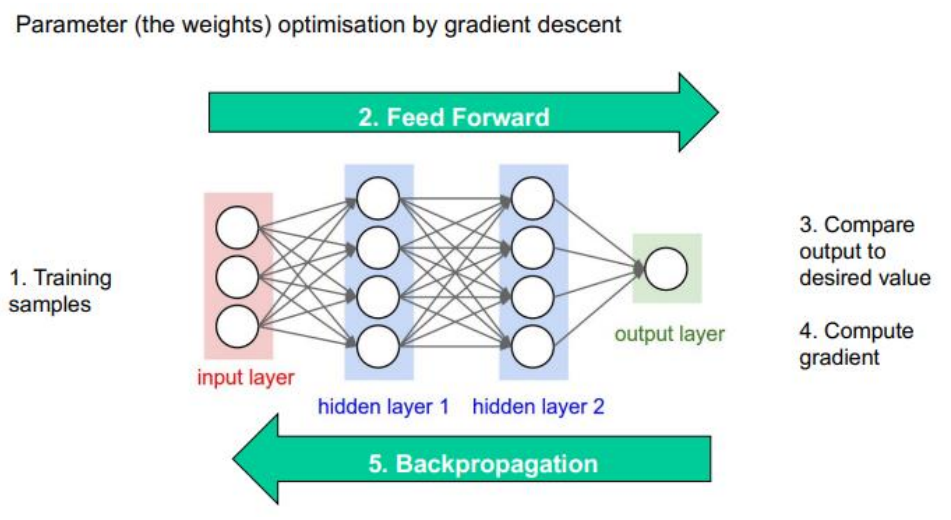
\includegraphics[width=\linewidth]{training_feed_forward_nn.png}    
\end{theorem}

\begin{example2}{Backpropagation Example}\\
Consider a simple neural network with one input, one hidden layer with two neurons, and one output neuron.
\begin{itemize}
    \item Input: $x = 0.5$
    \item Hidden layer weights: $w^{(1)}_{11} = 0.15, w^{(1)}_{21} = 0.25$
    \item Hidden layer biases: $b^{(1)}_1 = 0.35, b^{(1)}_2 = 0.45$
    \item Output layer weights: $w^{(2)}_{11} = 0.40, w^{(2)}_{12} = 0.50$
    \item Output layer bias: $b^{(2)}_1 = 0.60$
    \item Activation function: Sigmoid
    \item True output: $y = 0.75$
\end{itemize}
\tcblower
Forward pass:
\begin{align*}
z^{(1)}_1 &= w^{(1)}_{11} \cdot x + b^{(1)}_1 = 0.15 \cdot 0.5 + 0.35 = 0.425\\
a^{(1)}_1 &= \sigma(z^{(1)}_1) = \sigma(0.425) = 0.605\\
z^{(1)}_2 &= w^{(1)}_{21} \cdot x + b^{(1)}_2 = 0.25 \cdot 0.5 + 0.45 = 0.575\\
a^{(1)}_2 &= \sigma(z^{(1)}_2) = \sigma(0.575) = 0.640\\
z^{(2)}_1 &= w^{(2)}_{11} \cdot a^{(1)}_1 + w^{(2)}_{12} \cdot a^{(1)}_2 + b^{(2)}_1\\
&= 0.40 \cdot 0.605 + 0.50 \cdot 0.640 + 0.60 = 0.842 + 0.60 = 1.442\\
\hat{y} = a^{(2)}_1 &= \sigma(z^{(2)}_1) = \sigma(1.442) = 0.809
\end{align*}

Backpropagation:
\begin{align*}
\frac{\partial L}{\partial a^{(2)}_1} &= 2(a^{(2)}_1 - y) = 2(0.809 - 0.75) = 0.118\\
\frac{\partial a^{(2)}_1}{\partial z^{(2)}_1} &= a^{(2)}_1(1 - a^{(2)}_1) = 0.809 \cdot 0.191 = 0.154\\
\frac{\partial L}{\partial z^{(2)}_1} &= \frac{\partial L}{\partial a^{(2)}_1} \cdot \frac{\partial a^{(2)}_1}{\partial z^{(2)}_1} = 0.118 \cdot 0.154 = 0.018
\end{align*}

This gradient is then used to update the weights in the network.
\end{example2}

\raggedcolumns
\columnbreak

\begin{KR}{Simple NN Training}
    \begin{enumerate}
        \item Choose one sample from our dataset. We only operate on one sample at a time.
        \item Calculate all the partial derivatives of loss with respect to weights or biases.
        \item Use the update equation to update each weight and bias.
        \item Go back to step 1.
    \end{enumerate}
\end{KR}

\begin{example2}{Simple Neural Network Calculation}\\
Consider a simple neural network with:
\begin{itemize}
    \item $w_0=$ bias for all nodes $=0.2$
    \item $\operatorname{act}(z)= \begin{cases}z & \text { if } z \geq 0 \\ 0 & \text { otherwise }\end{cases}$
    \item Inputs: $i_1=3, i_2=-2$
\end{itemize}
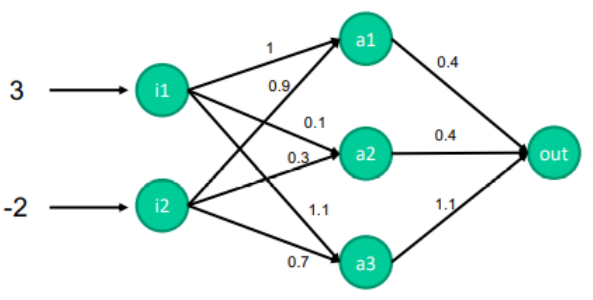
\includegraphics[width=0.6\linewidth]{simple_nn_example.png}
$$
\begin{gathered}
z_1=i_1 \cdot 1+i_2 \cdot 0.9+w_{a 1,0}=3 \cdot 1-2 \cdot 0.9+0.2=1.4 \\
a_1=\operatorname{act}(1.4)=1 \\
z_2=i_1 \cdot 0.1+i_2 \cdot 0.3+w_{a 2,0}=3 \cdot 0.1-2 \cdot 0.3+0.2=-0.1 \\
a_2=\operatorname{act}(-0.1)=0 \\
z_3=i_1 \cdot 1.1+i_2 \cdot 0.7+w_{a 3,0}=3 \cdot 1.1-2 \cdot 0.7+0.2=2.1 \\
a_3=\operatorname{act}(2.1)=1
\end{gathered}
$$

\end{example2}

\raggedcolumns
\columnbreak

\subsection{Neural Network Architectures}

Neural networks come in various architectures, each designed for specific types of data or tasks.

\begin{definition}{Common Neural Network Architectures}
\begin{itemize}
    \item \textbf{Fully Connected (Dense) Network}: Each neuron is connected to all neurons in adjacent layers
    \item \textbf{Convolutional Neural Network (CNN)}: Uses convolutional layers to process grid-like data (e.g., images)
    \item \textbf{Recurrent Neural Network (RNN)}: Contains loops to persist information, suitable for sequential data
    \item \textbf{Long Short-Term Memory (LSTM)}: A special type of RNN that can learn long-term dependencies
    \item \textbf{Transformer}: Uses attention mechanisms, effective for sequential data like text
\end{itemize}
\end{definition}

\begin{concept}{Convolutional Neural Networks}
CNNs are specialized for processing grid-like data such as images:
\begin{itemize}
    \item \textbf{Convolutional layers}: Apply filters to detect local patterns
    \item \textbf{Pooling layers}: Reduce spatial dimensions while retaining important features
    \item \textbf{Parameter sharing}: Same filter applied across the entire input
    \item \textbf{Local connectivity}: Each neuron connects to a small region of the input
\end{itemize}
These properties make CNNs highly effective for tasks like image classification, object detection, and image segmentation.
\end{concept}

\begin{concept}{Recurrent Neural Networks}
RNNs are designed for sequential data:
\begin{itemize}
    \item Each neuron receives input from the current sample and its own previous output
    \item This creates a form of memory that captures dependencies across time steps
    \item Useful for tasks like time series prediction, speech recognition, and language modeling
    \item Variants like LSTM and GRU address the vanishing gradient problem in standard RNNs
\end{itemize}
\end{concept}

\subsubsection{Preventing Overfitting}

Overfitting occurs when a model learns the training data too well, including its noise, and fails to generalize to new data. Several techniques can prevent this issue in neural networks.

\mult{2}
\begin{concept}{Dealing with Overfitting in Neural Networks}
Techniques to prevent overfitting include:
\begin{itemize}
    \item \textbf{Dropout}: Randomly deactivate neurons during training
    \item \textbf{Early Stopping}: Stop training when performance on validation set starts to degrade
    \item \textbf{Data Augmentation}: Create new training samples by applying transformations
    \item \textbf{Regularization}: Add penalty terms for large weights
\end{itemize}
\end{concept}

\begin{definition}{Early Stopping}
Early stopping prevents overfitting by monitoring performance on a validation set:
\begin{itemize}
    \item Train the model and evaluate on validation set periodically
    \item Stop training when validation error starts to increase
    \item Use the model parameters from the point with best validation performance
\end{itemize}
\end{definition}

\begin{definition}{Dropout}
Dropout is a regularization technique that prevents overfitting in neural networks:
\begin{itemize}
    \item During training, randomly deactivate a fraction of neurons in each layer
    \item Each forward and backward pass uses a different randomly dropped network
    \item Forces the network to learn redundant representations
    \item During inference, all neurons are used (with scaled activations)
\end{itemize}
\end{definition}



\begin{definition}{Data Augmentation}
Data augmentation increases the effective size of the training dataset:
\begin{itemize}
    \item For images: rotations, flips, crops, color adjustments
    \item For text: synonym replacement, back-translation
    \item For audio: time stretching, pitch shifting, masking
\end{itemize}
\end{definition}

\multend

\begin{concept}{Vanishing and Exploding Gradient Problems}
In deep networks, gradients can become very small (vanishing) or very large (exploding) as they propagate through the network:
\begin{itemize}
    \item \textbf{Vanishing gradients}: Parameters in early layers change very slowly or not at all
    \item \textbf{Exploding gradients}: Parameters in early layers change dramatically, causing instability
    \item \textbf{Causes}: Repeated multiplication of values less than 1 (vanishing) or greater than 1 (exploding)
\end{itemize}
Solutions include:
\begin{itemize}
    \item Better activation functions (ReLU, Leaky ReLU)
    \item Weight initialization techniques (Xavier, He initialization)
    \item Batch normalization
    \item Residual connections (skip connections)
\end{itemize}
\end{concept}

\begin{KR}{Implementing Dropout}
\paragraph{During training}
\begin{itemize}
    \item For each training batch, generate a binary mask for each layer with dropout
    \item Set a dropout rate (typically 0.2-0.5) representing the fraction of neurons to drop
    \item Multiply activations by the mask to zero out dropped neurons
    \item Scale remaining activations by $\frac{1}{1-\text{dropout\_rate}}$ to maintain same expected value
\end{itemize}

\paragraph{During testing/inference}
\begin{itemize}
    \item Use all neurons without dropout
    \item No scaling needed if scaling was done during training
\end{itemize}

\paragraph{Implementation considerations}
\begin{itemize}
    \item Apply dropout after activation functions
    \item Use different dropout rates for different layers (typically higher for layers with more neurons)
    \item Don't apply dropout to the output layer
\end{itemize}
\end{KR}




\subsection{Hyperparameter Tuning}

Hyperparameters are settings that control the training process and model architecture. Choosing optimal values is crucial for model performance.

\begin{KR}{Choosing Hyperparameters for Neural Networks}
\paragraph{Architecture design}
\begin{itemize}
    \item Number of layers: Start small and increase gradually
    \item Neurons per layer: Powers of 2 (64, 128, 256) work well; larger for complex tasks
    \item Activation functions: ReLU for hidden layers, softmax for multi-class output
\end{itemize}

\paragraph{Training parameters}
\begin{itemize}
    \item Learning rate: Start with 0.01 or 0.001 and tune using learning rate finder
    \item Batch size: 32, 64, or 128 for most tasks; larger if memory allows
    \item Optimizer: Adam is a good default choice
    \item Epochs: Use early stopping with patience
\end{itemize}

\paragraph{Regularization}
\begin{itemize}
    \item Dropout rate: 0.2-0.5 depending on layer size
    \item Weight decay (L2 regularization): 1e-4 is a reasonable starting point
    \item Early stopping patience: 10-20 epochs
\end{itemize}

\paragraph{Advanced techniques}
\begin{itemize}
    \item Learning rate schedules: Reduce on plateau or cosine annealing
    \item Batch normalization: Apply before activation functions
    \item Skip connections: Use for networks deeper than 10 layers
\end{itemize}
\end{KR}

\mult{2}

\begin{concept}{Cross-Validation for Neural Networks}\\
Cross-validation helps find optimal hyperparameters:
\begin{itemize}
    \item Split data into training, validation, and test sets
    \item Train models with different hyperparameter combinations
    \item Evaluate each model on validation set
    \item Select hyperparameters that yield best validation performance
    \item Final evaluation on test set
\end{itemize}
Unlike traditional k-fold cross-validation, neural networks often use a single validation split due to computational constraints.
\end{concept}

\begin{example}{Digit Recognition with Neural Networks}
Consider the MNIST dataset of handwritten digits:
\begin{itemize}
    \item Input: 28x28 pixel grayscale images (784 features)
    \item Output: 10 classes (digits 0-9)
    \item Network architecture:
    \begin{itemize}
        \item Input layer: 784 neurons
        \item Hidden layer 1: 128 neurons with ReLU activation
        \item Hidden layer 2: 64 neurons with ReLU activation
        \item Output layer: 10 neurons with softmax activation
    \end{itemize}
    \item Training:
    \begin{itemize}
        \item Loss function: Categorical cross-entropy
        \item Optimizer: Adam with learning rate 0.001
        \item Batch size: 64
        \item Epochs: 20 with early stopping
    \end{itemize}
    \item Results:
    \begin{itemize}
        \item Training accuracy: 99.2\%
        \item Validation accuracy: 98.1\%
    \end{itemize}
\end{itemize}
\end{example}

\multend

\raggedcolumns
\columnbreak

\subsection{Advanced Topics}

Neural networks continue to evolve with advanced techniques that improve performance, efficiency, and applicability to various domains.

\begin{concept}{Transfer Learning}\\
Transfer learning leverages knowledge from pre-trained models:
\begin{itemize}
    \item Start with a model trained on a large dataset
    \item Remove the final layer(s) and replace with new layers
    \item Either freeze pre-trained layers or fine-tune them with a small learning rate
    \item Requires much less data than training from scratch
    \item Common in computer vision (ResNet, VGG) and NLP (BERT, GPT)
\end{itemize}
\end{concept}

\begin{definition}{Batch Normalization}\\
Batch normalization normalizes the inputs of each layer:
\begin{itemize}
    \item Normalizes activations to have mean 0 and variance 1
    \item Reduces internal covariate shift
    \item Allows higher learning rates
    \item Acts as a regularizer
    \item Applied before or after activation functions
\end{itemize}
\end{definition}

\begin{concept}{Advanced Optimizers}\\
Beyond standard gradient descent, advanced optimizers improve training:
\begin{itemize}
    \item \textbf{Momentum}: Adds a fraction of previous update to current update
    \item \textbf{RMSprop}: Adapts learning rates based on recent gradients
    \item \textbf{Adam}: Combines momentum and RMSprop
    \item \textbf{AdamW}: Adam with decoupled weight decay
\end{itemize}
\end{concept}

\begin{KR}{Implementing Transfer Learning}
\paragraph{Select pre-trained model}
\begin{itemize}
    \item Choose model trained on a relevant domain
    \item Consider model size, accuracy, and compatibility
    \item Common options: ResNet, VGG, EfficientNet for images; BERT, GPT for text
\end{itemize}

\paragraph{Prepare the model}
\begin{itemize}
    \item Load pre-trained weights
    \item Remove the output layer (and possibly some layers before it)
    \item Add new layers specific to your task
\end{itemize}

\paragraph{Training approach}
\begin{itemize}
    \item Feature extraction: Freeze pre-trained layers, train only new layers
    \item Fine-tuning: Train the entire network with a small learning rate
    \item Progressive fine-tuning: Gradually unfreeze more layers
\end{itemize}

\paragraph{Adapt to your data}
\begin{itemize}
    \item Ensure input preprocessing matches pre-trained model
    \item Consider domain adaptation techniques if domains differ significantly
    \item Use appropriate regularization for new layers
\end{itemize}
\end{KR}

\begin{example2}{Practical Neural Network Project}\\
Consider an image classification task to identify plant diseases from leaf images:
\begin{itemize}
    \item Dataset: 5,000 images across 10 disease categories
    \item Limited computational resources
\end{itemize}
\tcblower
Solution approach using transfer learning:
\begin{itemize}
    \item Base model: Pre-trained ResNet50 (trained on ImageNet)
    \item Remove top classification layer
    \item Add custom layers:
    \begin{itemize}
        \item Global average pooling
        \item Dropout layer (rate=0.3)
        \item Dense layer with 256 neurons and ReLU activation
        \item Final layer with 10 neurons and softmax activation
    \end{itemize}
    \item Training strategy:
    \begin{itemize}
        \item First stage: Freeze ResNet layers, train only custom layers (5 epochs)
        \item Second stage: Unfreeze last 30 ResNet layers, train entire model with small learning rate (0.0001) for 15 epochs
    \end{itemize}
    \item Data augmentation:
    \begin{itemize}
        \item Random rotations (±20°)
        \item Horizontal and vertical flips
        \item Small zoom and brightness variations
    \end{itemize}
    \item Results: 96.5\% accuracy on test set, compared to 85\% when training from scratch
\end{itemize}
\end{example2}

\begin{concept}{Model Interpretability}\\
Techniques to understand neural network decisions:
\begin{itemize}
    \item \textbf{Feature importance}: Quantifying the impact of each input feature
    \item \textbf{Activation visualization}: Examining neuron activations for different inputs
    \item \textbf{Saliency maps}: Highlighting regions of input that most influence the output
    \item \textbf{LIME (Local Interpretable Model-agnostic Explanations)}: Approximating the model locally with an interpretable model
    \item \textbf{SHAP (SHapley Additive exPlanations)}: Assigning each feature an importance value
\end{itemize}
Interpretability helps build trust, debug models, and identify potential biases.
\end{concept}

\begin{KR}{Debugging Neural Networks}
\paragraph{Diagnose learning problems}
\begin{itemize}
    \item Monitor training and validation losses
    \item If validation loss increases while training loss decreases: Overfitting
    \item If both losses plateau at high values: Underfitting
    \item If both losses are unstable: Learning rate may be too high
\end{itemize}

\paragraph{Check gradients}
\begin{itemize}
    \item Inspect gradient magnitudes; very large or very small values indicate problems
    \item Test with gradient clipping to prevent exploding gradients
    \item Verify with numerical gradient checking in critical cases
\end{itemize}

\paragraph{Analyze model predictions}
\begin{itemize}
    \item Examine confusion matrix to identify patterns in misclassifications
    \item Look at the most confidently wrong predictions
    \item Test with simpler inputs to verify basic functionality
\end{itemize}

\paragraph{Simplify and rebuild}
\begin{itemize}
    \item Start with a minimal working model
    \item Add complexity incrementally
    \item Establish baseline performance with simple models
    \item Verify each component individually
\end{itemize}
\end{KR}

%TODO: Add simple neural network diagram showing the specific calculation example with values